\documentclass[Softwaredesign/Softwaredesign_main.tex]{subfiles}

\begin{document}
    \section{CoinDetector software design}\label{sec:coindetectorSoftwareDesign}
    Our design required a way to detect coins as well as a way to handle the coins after they had entered the system.
    In this section the design of the CoinDetector as well as some choices that where made along the way.\\
    The CoinDetector software consists of 4 different modules, they are the CoinDetector itself, MotorControl, UART and I2C.
    The CoinDetector is the main logic of the software, it contains the state machine to whether to keep the coin or reject it using the MotorControl.
    It also uses the UART and I2C functions to signal to the rest of the system what state the machine is in.


    \subsection{CoinDetector Design choices}\label{subsec:coindetectorDesignChoices}
    When designing the CoinSensor we looked at a few different approaches.
    The ideas we where considering where some kind of light sensor or a leaver type switch that the coin
    would hit before it entered the system, before we ended up on the final design of using a simple short circuit.


    \subsection{CoinDetector with short circuit design}\label{subsec:coindetectorWithShortCircuitDesign}
    \begin{figure}[H]
    \centering
    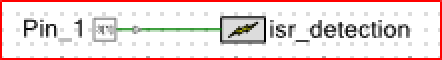
\includegraphics[width=0.5\textwidth]{Softwaredesign/CoinSensor/graphics/TopDesign-CoinDetector.png}
    \caption{PSoC top design CoinDetector}
    \label{fig:CoinDetector_PSoC_Design}
    \end{figure}
    The software for the detector is pretty simple.
    It consists of a simple interrupt.
    The interrupt disables future interrupts then calls the appropriate functions depending on what state the dispenser is in.
    If the dispenser is in the off state it calls the required motor functions to reject the coin,
    re-enables the interrupt then goes back to waiting.
    If the dispenser is in the on state it sends a message to the gamecontroller via I2C then calls the required motor functions,
    re-enables the interrupt then goes back to waiting.

    \subsection{Motor Control Design}\label{subsec:motorControlDesign}
    \begin{figure}[H]
    \centering
    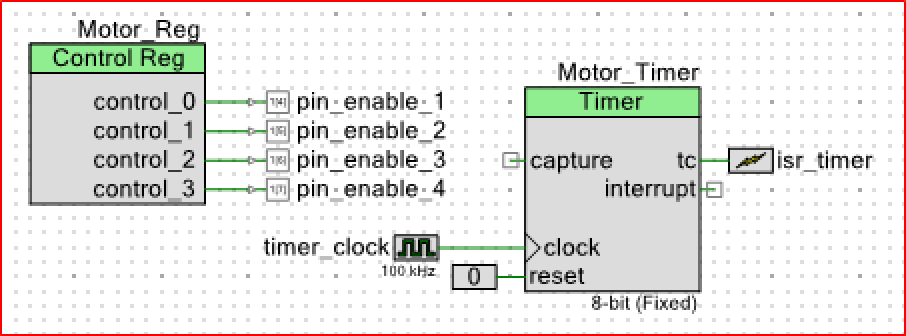
\includegraphics[width=\textwidth]{Softwaredesign/CoinSensor/graphics/TopDesign-MotorControl.png}
    \caption{PSoC top design MotorControl}
    \label{fig:MotorControl_PSoC_Design}
    \end{figure}
    This is the motor diver that will control the coin accept and reject functionality as well as the ball dispenser.
    It is made using a control register that is connected to a stepper motor and there is a timer used to control the speed of the motor.
    The register is then modified to rotate the motor in fullstep mode.
    The driver also has functions to rotate the motor a certain amount of degrees. 

\end{document}